\subsection{Geometry vs Volume}

\subsubsection{Geometry and Image Segmentation}
\subsubsubsection{\textbf{Segmentation}}
In our data set there were 181 slices each containing an image with the dimensions 256x256.  For each slice the segmentation described in the segmentation section of the report was performed to identify each of the known tissues within our dataset.  Figure \ref{fig:resultsHistogram} shows an example the histogram distribution along with their corresponding MRI. Note the distinct peaks of the histogram which corresponds the the distinct known tissues of the brain.\\ 

\begin{figure}[h]
  \centering
  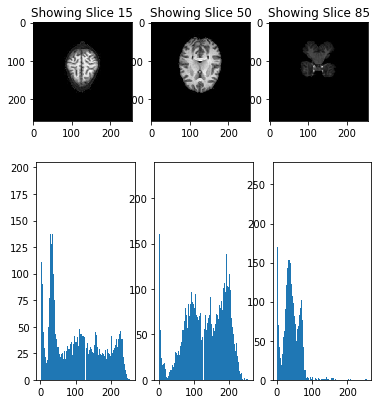
\includegraphics[width=\linewidth]{pictures/resultsHistogram.png}
  \caption{Brain slices of MRI with their corresponding histogram distribution.}
  \label{fig:resultsHistogram}
\end{figure}

Results of the manual seed region growing techniques and morphological filters can be seen in figure \ref{fig:resultsSegmentation}.

\begin{figure}[h]
  \centering
  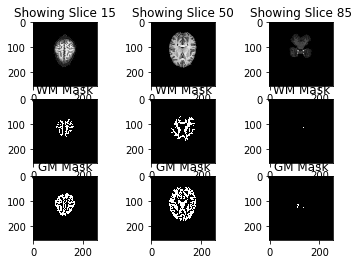
\includegraphics[width=\linewidth]{pictures/resultsSegmentation.png}
  \caption{\textbf{Top Row:} Original MRI. \textbf{Middle Row:}White matter mask. \textbf{Bottom Row:}Gray matter mask.}
  \label{fig:resultsSegmentation}
\end{figure}

We applied this technique not only for the regular brain but also for a brain which contains a tumor.  The following set of figures shows examples slices as well as their resultant class labels and individual mask layers.\\

\begin{figure}[h]
  \centering
  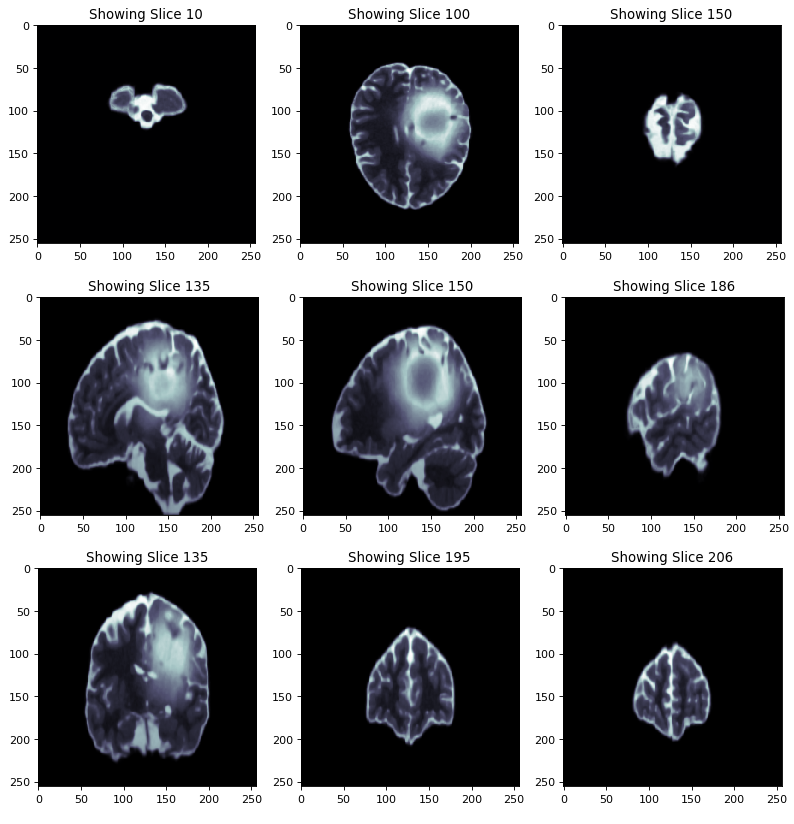
\includegraphics[width=\linewidth]{pictures/originalMRI.png}
  \caption{Original MRI slices in different views.  From top to bottom they are sliced in the axial, sagittal and coronal planes.}
  \label{fig:originalMRI}
\end{figure}

\begin{figure}[h]
  \centering
  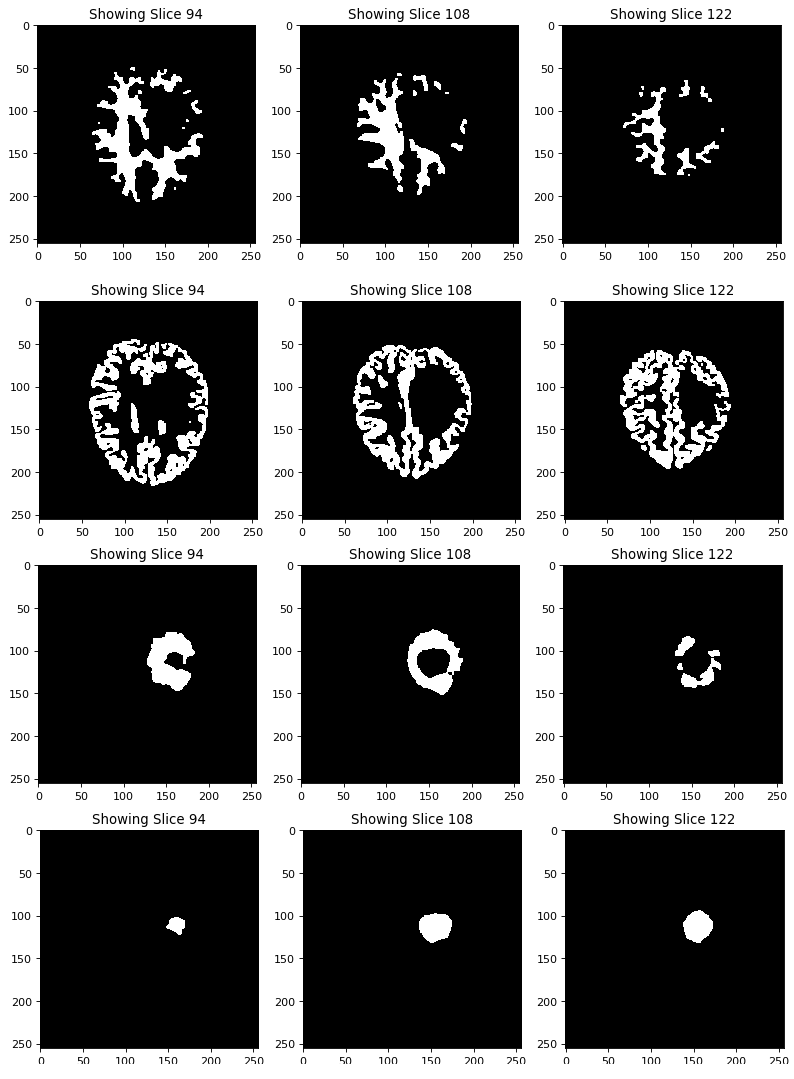
\includegraphics[width=\linewidth]{pictures/resultantMasks.png}
  \caption{Generated masks for each of the known tissue classes in our dataset.  From top to bottom they are: gray matter, white matter, abnormal tissue, and tumor.}
  \label{fig:resultantMasks}
\end{figure}

Even though we applied morphological filters we can still see some noise within the images, specifically the speckle effects in the gray matter and some holes in the white matter masks.\\  

\begin{figure}[h]
  \centering
  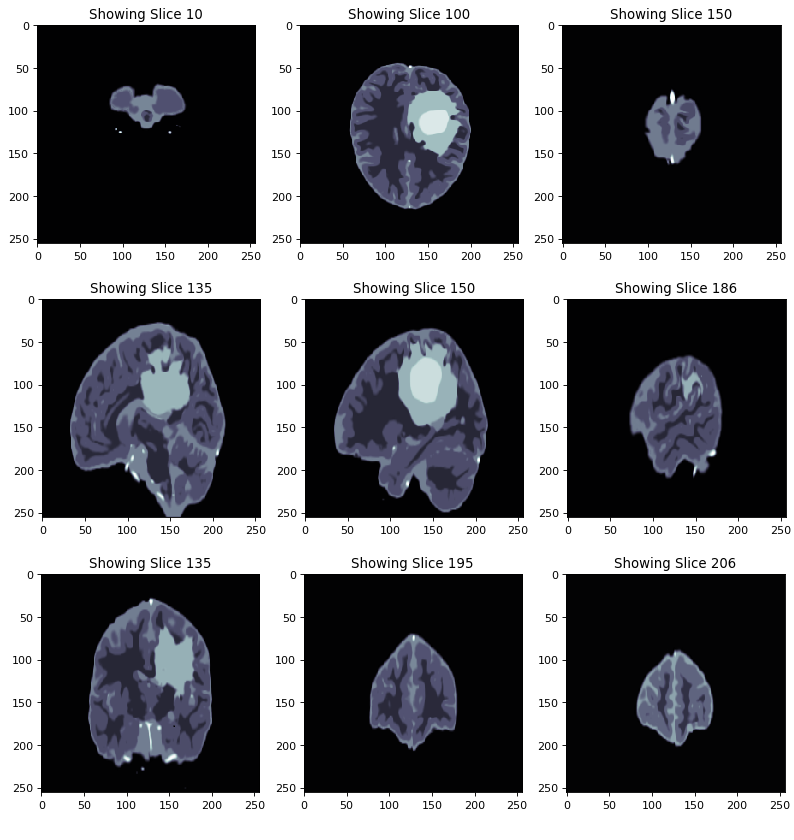
\includegraphics[width=\linewidth]{pictures/labeledMasks.png}
  \caption{Various slices and views of each of the coloured masks as found in the histogram.}
  \label{fig:labeledMasks}
\end{figure}

Each unique colour corresponds to a unique known tissue type.  By looking at various views you can get a picture as to where the tumor maybe located.  To create contrast between each distinct region we proposed the following colouring scheme.

\begin{figure}[h]
  \centering
  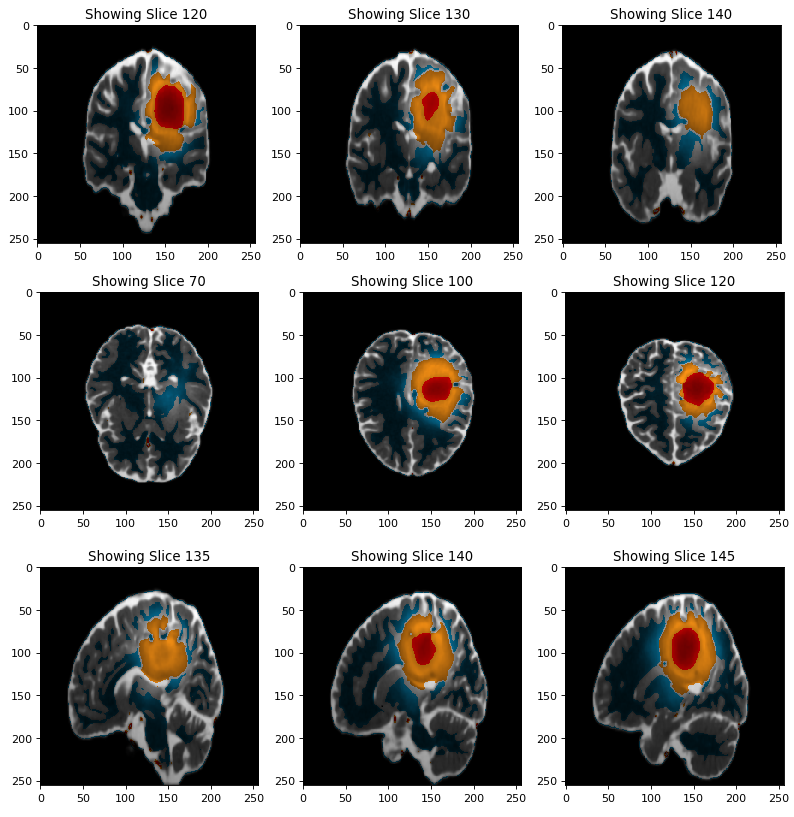
\includegraphics[width=\linewidth]{pictures/colourCodedRegions.png}
  \caption{Colour coded regions of the brain}
  \label{fig:colourCodedRegions}
\end{figure}

\begin{table}[h]
\centering
\begin{tabular}{|r|l|l|l|}
\hline
Tissue & R & \multicolumn{1}{c|}{G} & B \\ \hline
White & 7 & \multicolumn{1}{c|}{150} & 204 \\ \hline
Gray & 204 & 204 & 204 \\ \hline
Abnormal Tissue & 203 & 119 & 17 \\ \hline
Tumor & 203 & 2 & 2 \\ \hline
\end{tabular}
\caption{RGB values of each of the tissue types.}
\label{table:RGBValues}
\end{table}

Notice that for each of the tissue types they can be clearly distinguish from each other. 

\subsubsubsection{\textbf{Geometry Generation}}
From a far it may seem that the models are what we expect but looking at the smaller object such as the tumor and the abnormal tissue it is clear that the resolution of the models are directly correlated with the number of slices within the DICOM file.  The marching cube algorithm generates these step wise artifacts which are the depth of the each slice within the MRI.  Because we can't use smoothing techniques, the only remedy to this is to increase the number of slices.  This will increase the computational cost and time to create a model for printing.  For most use cases we think that this is okay in the long run for holographic prints.  But for regular clinical practice like in the operating room or emergency care this is not feasible.  Nevertheless we prove that it is possible to perform semi-automatic segmentation in conjunction with marching cube algorithm to develop geometry.\\

\begin{figure}[h]
  \centering
  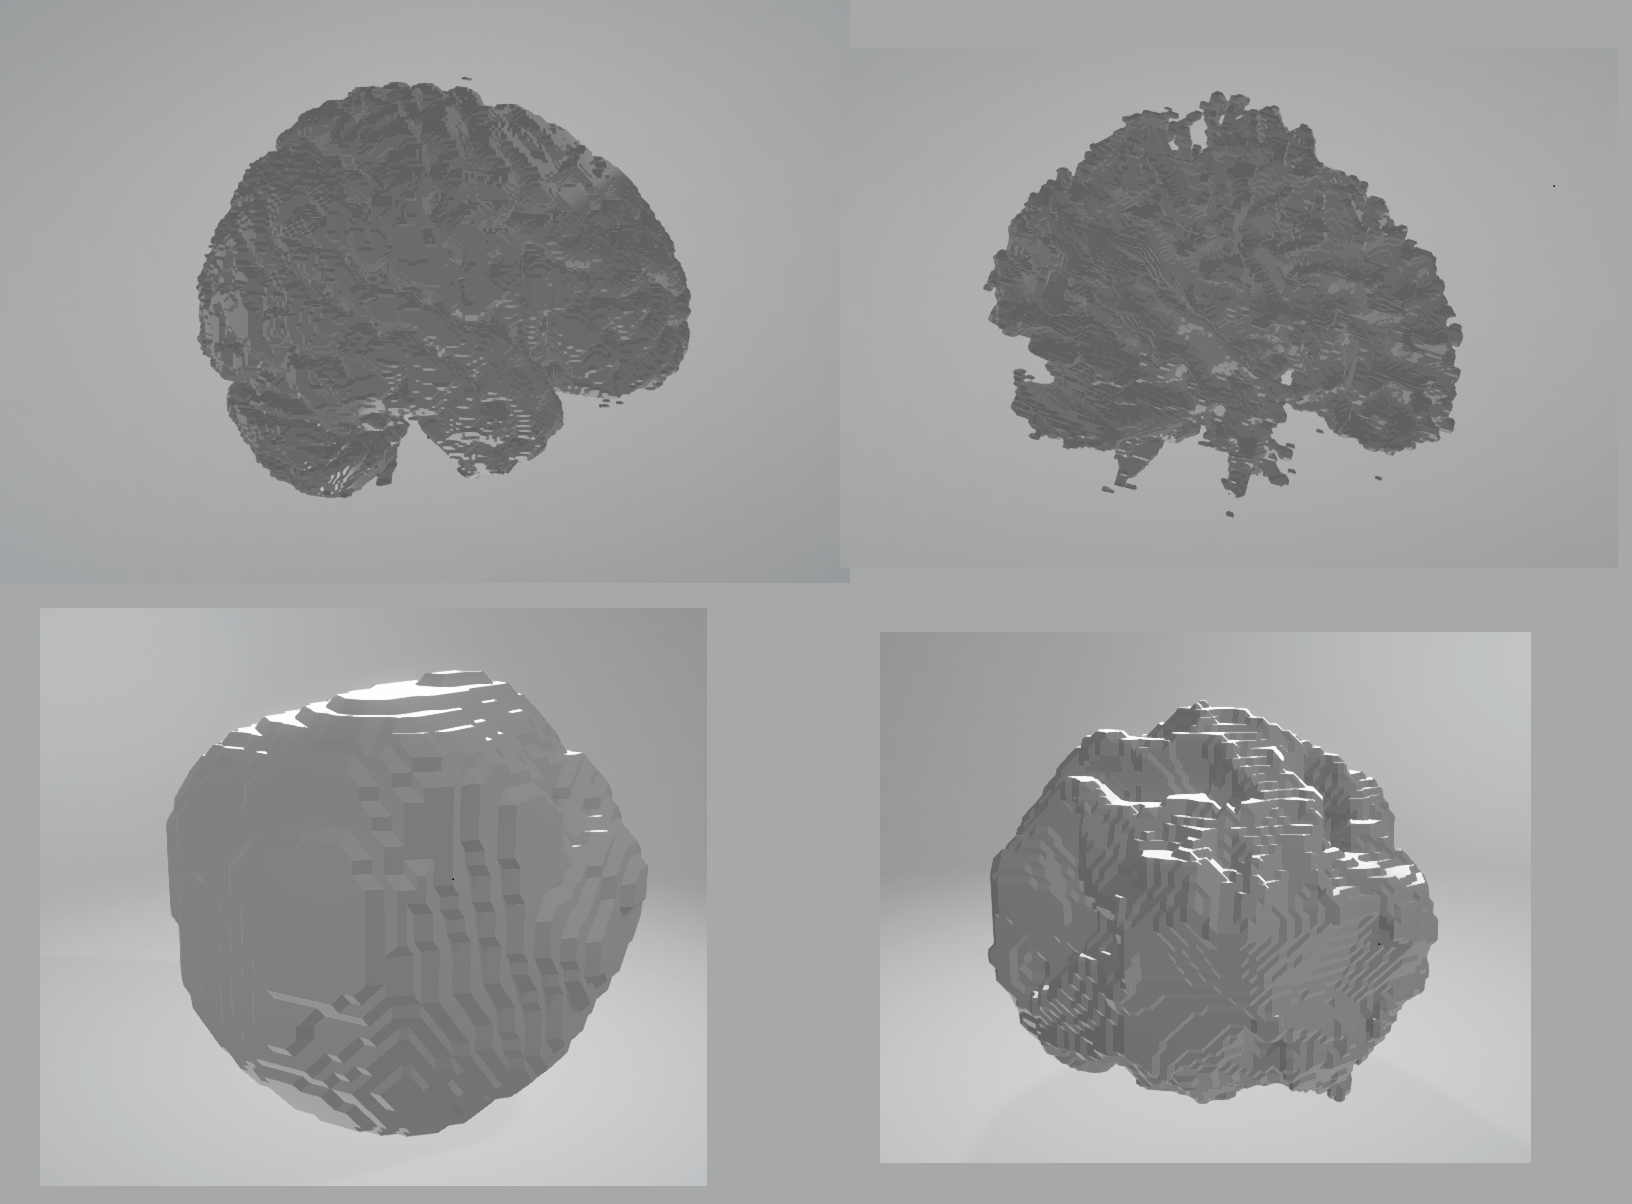
\includegraphics[width=\linewidth]{pictures/resultsMarchingCube.PNG}
  \caption{\textbf{Top Left:} Gray matter \textbf{Top Right:} White matter \textbf{Bottom Left:} Tumor \textbf{Bottom Right:} Abnormal tissue.}
  \label{fig:resultsMarchingCube}
\end{figure}

\begin{figure}[h]
 \centering % avoid the use of \begin{center}...\end{center} and use \centering instead (more compact)
 
\includegraphics[width=\columnwidth]{pictures/general-model.png}
 \caption{Current State}
 \label{fig:general-model}
\end{figure}

\subsubsection{Volume Observations: Opaque and Translucent Views}
The opaque views create a three dimensional form in the viewing space, with defined markings on the brain surface. In figures \ref{fig:noalphared-lateral} through \ref{fig:alphared-front}, our rendering sample depicts an applied red transmission colour.

% \begin{figure}[ht]
%  \centering % avoid the use of \begin{center}...\end{center} and use \centering instead (more compact)
%  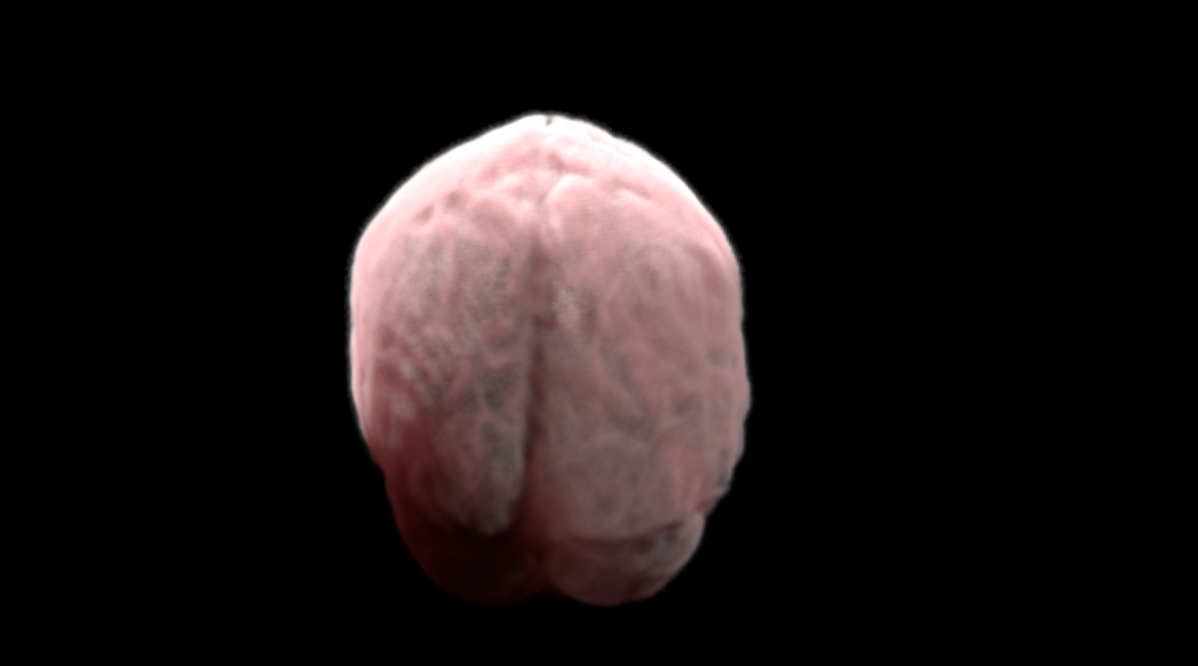
\includegraphics[width=\columnwidth]{pictures/bt-noalphared-front.png}
%  \caption{Opaque MRI Render. Front view.}
%  \label{fig:noalphared-front}
% \end{figure}

\begin{figure}[h]
 \centering % avoid the use of \begin{center}...\end{center} and use \centering instead (more compact)
 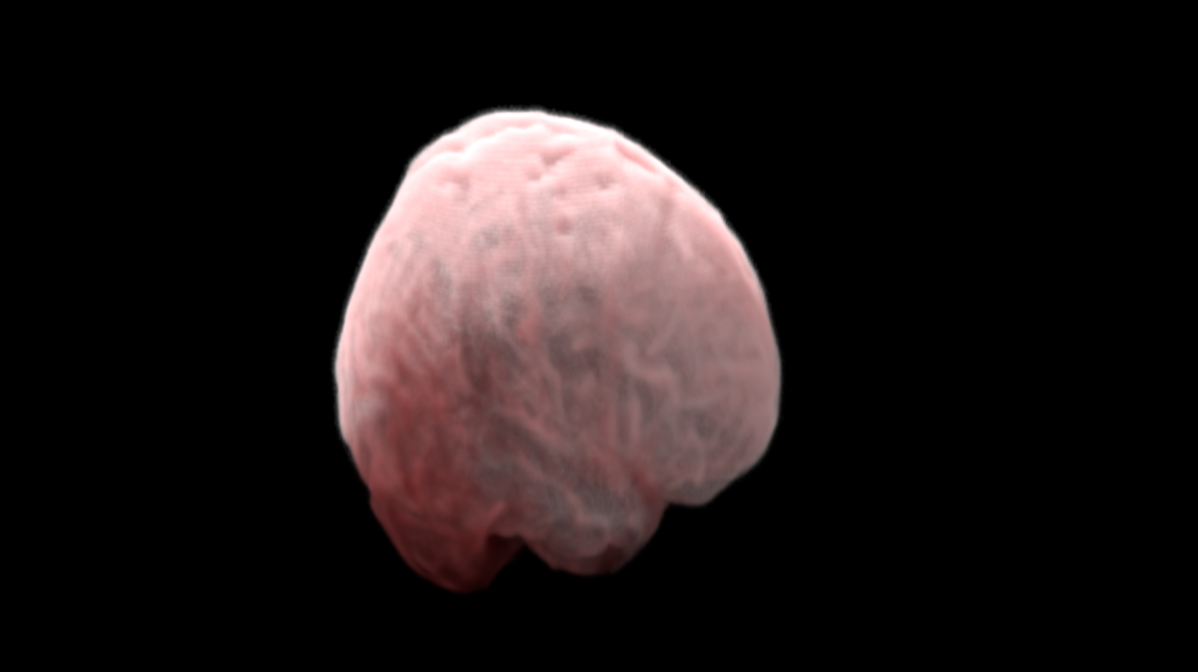
\includegraphics[width=\columnwidth]{pictures/bt-noalphared-lateral.png}
 \caption{Opaque MRI Render. Lateral view.}
 \label{fig:noalphared-lateral}
\end{figure}

\begin{figure}[h]
 \centering % avoid the use of \begin{center}...\end{center} and use \centering instead (more compact)
 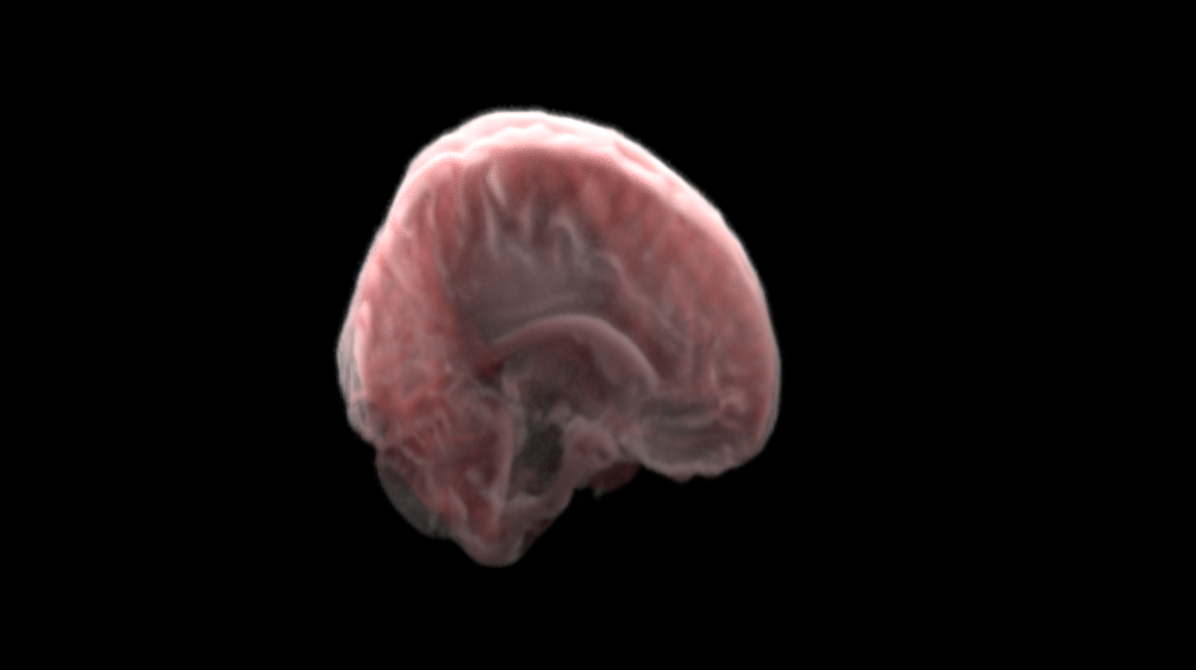
\includegraphics[width=\columnwidth]{pictures/bt-noalphared-lateral-slice.png}
 \caption{Opaque MRI Render. Lateral slice view.}
 \label{fig:noalphared-lateral-slice}
\end{figure}

\begin{figure}[h]
 \centering % avoid the use of \begin{center}...\end{center} and use \centering instead (more compact)
 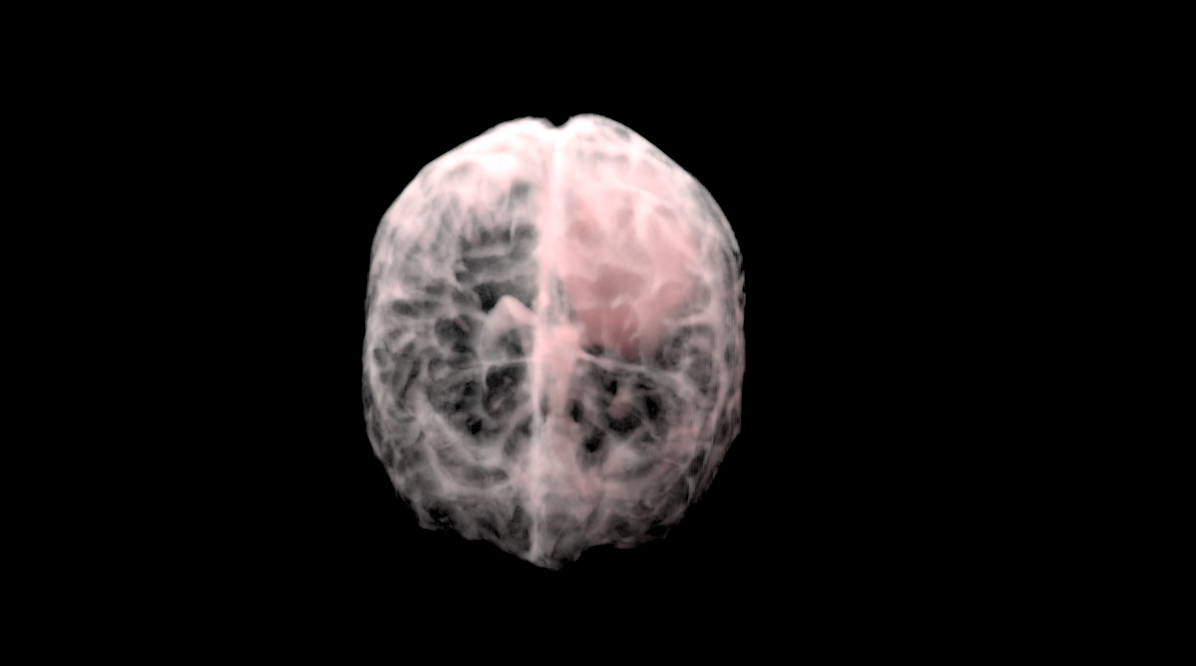
\includegraphics[width=\columnwidth]{pictures/bt-alphared-front.png}
 \caption{Translucent MRI Render. Front view.}
 \label{fig:alphared-front}
\end{figure}

\begin{figure}[h]
 \centering % avoid the use of \begin{center}...\end{center} and use \centering instead (more compact)
 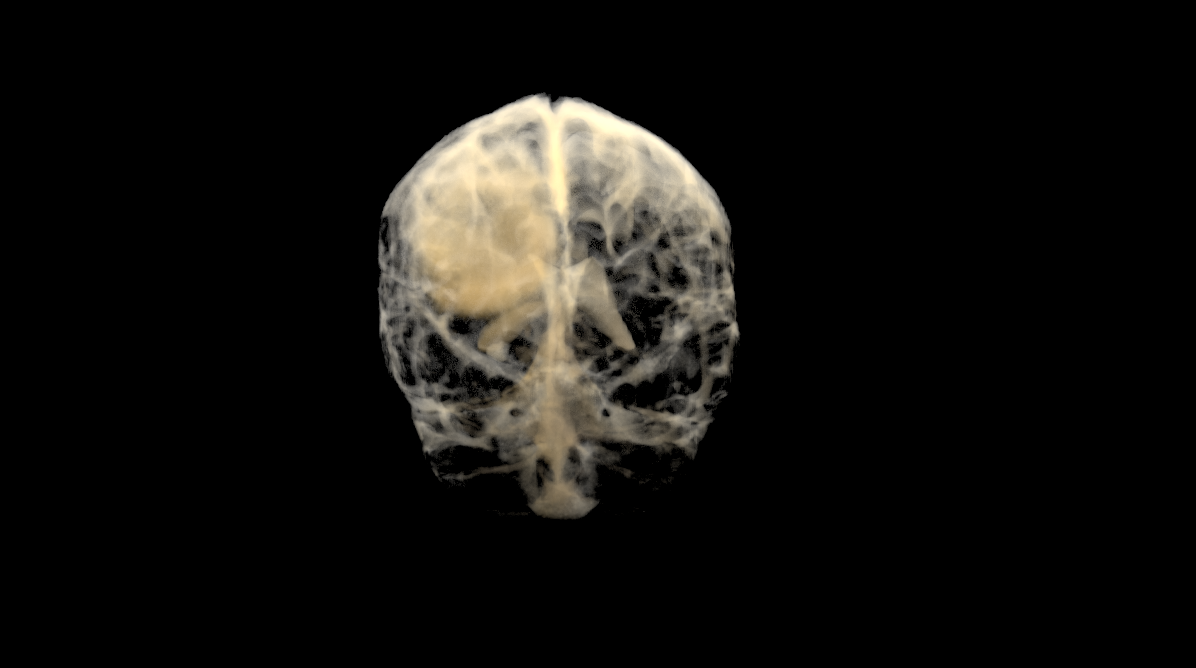
\includegraphics[width=\columnwidth]{pictures/bt-alphalimon-back.png}
 \caption{Translucent MRI Render. Front view.}
 \label{fig:alphared-front}
\end{figure}

Slight opaque regions are revealed from the top down in opaque slices. Translucent slices have a more crystallized look and feel to the image when sliced, however the TC regions are much more prominent.